% fig4-composed-cost.tex — §7 composed cost waterfall (RC-07)
% Data source: data/aggregated/composed-cost.csv + routing-baseline-results.csv
%
% Four levels (cost remaining as % of no-cache baseline):
%   0: No-caching baseline:            100.0% remaining (0% saved)
%   1: + Prefix-cache:                  21.4% remaining (78.6% saved)
%   2: + Prefix + plan-cache (n=40):    18.2% remaining (81.8% saved)
%   3: + Prefix + plan-cache + routing: 17.8% remaining (82.2% saved)
%
% Sources:
%   composed-cost.csv: prefix_only_savings_pct=78.6
%   plancache-summary.csv: composed_cost_reduction_vs_prefix_only=0.8181 (synthetic n=40)
%   routing-baseline-results.csv: semantic-sim total_cost_saved_usd=0.28925 over 49 turns
%     => ~2.3% marginal on remaining 18.2% => composed ~82.2%

\begin{figure}[ht]
\centering
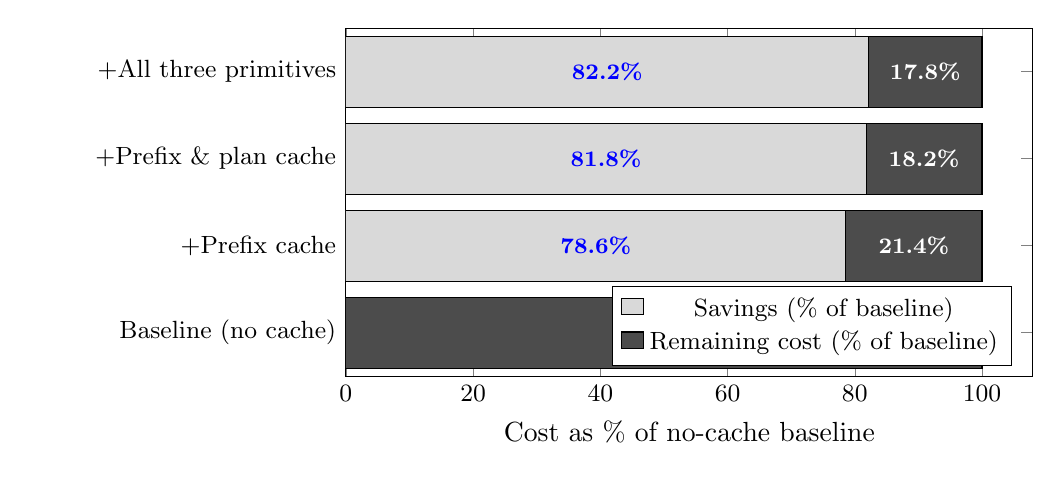
\begin{tikzpicture}
\begin{axis}[
  xbar stacked,
  width=0.85\textwidth,
  height=6cm,
  bar width=0.9cm,
  xmin=0, xmax=108,
  ymin=-0.5, ymax=3.5,
  ytick={0,1,2,3},
  yticklabels={
    {Baseline (no cache)},
    {$+$Prefix cache},
    {$+$Prefix \& plan cache},
    {$+$All three primitives}
  },
  yticklabel style={font=\small, align=right, text width=3.8cm},
  xlabel={Cost as \% of no-cache baseline},
  xticklabel style={font=\small},
  xtick={0,20,40,60,80,100},
  legend style={
    at={(0.97,0.03)},
    anchor=south east,
    legend columns=1,
    font=\small,
    draw=black,
  },
  nodes near coords,
  nodes near coords align={center},
  every node near coord/.append style={font=\footnotesize\bfseries},
  point meta=explicit symbolic,
]

% Saved portion (light fill)
\addplot+[fill=black!15, draw=black] coordinates {
  (0.0,  0) [0\%]
  (78.6, 1) [78.6\%]
  (81.8, 2) [81.8\%]
  (82.2, 3) [82.2\%]
};

% Remaining cost (dark fill)
\addplot+[
  fill=black!70,
  draw=black,
  every node near coord/.append style={color=white},
] coordinates {
  (100.0, 0) [100\%]
  (21.4,  1) [21.4\%]
  (18.2,  2) [18.2\%]
  (17.8,  3) [17.8\%]
};

\legend{Savings (\% of baseline), Remaining cost (\% of baseline)}
\end{axis}
\end{tikzpicture}

\caption{%
  Composed cost reduction across three primitives (expressed as \% of
  no-cache baseline).
  Prefix caching alone achieves 78.6\,\% savings.
  Adding plan caching (synthetic fixture, $n=40$) contributes a further 3.2\,pp
  to 81.8\,\%.
  Per-turn routing (semantic-similarity, LOO-CV) adds a marginal $\approx$0.4\,pp,
  for a composed figure of 82.2\,\%.
  Per-turn routing and agentic plan caching are complementary; their gains
  compound on the residual cost fraction.
  Sources: \texttt{data/aggregated/composed-cost.csv},
  \texttt{data/aggregated/plancache-summary.csv},
  \texttt{data/aggregated/routing-baseline-results.csv}.%
}
\label{fig:composed-cost}
\end{figure}
